\begin{figure}[t]\centering
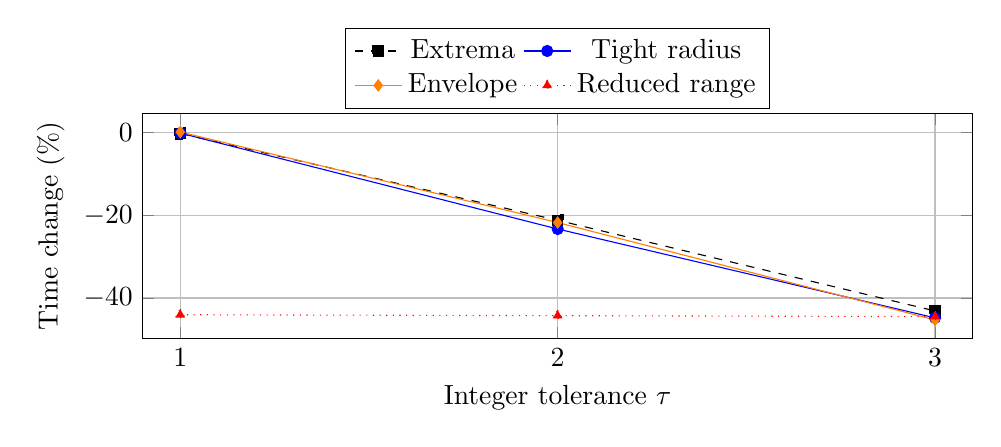
\begin{tikzpicture}
\begin{axis}[width=\columnwidth,height=1.75in,xmin=.9,xmax=3.1,xtick={1,2,3},xlabel={Integer tolerance $\tau$},ylabel={Time change (\%)},grid=major,legend style={font=\normalsize,at={(0.5,1.02)},anchor=south,legend columns=2},tick label style={font=\normalsize},label style={font=\normalsize}]
\addplot[black,dashed,mark=square*] coordinates {(1,-0.206836266765964) (2,-21.200167963546683) (3,-43.14758628598805)};\addlegendentry{Extrema}
\addplot[blue,mark=*] coordinates {(1,-0.11006956666549754) (2,-23.316582071330778) (3,-44.80995521596279)};\addlegendentry{Tight radius}
\addplot[orange,mark=diamond*] coordinates {(1,0.146060515430102) (2,-21.747187597103316) (3,-45.309245997001256)};\addlegendentry{Envelope}
\addplot[red,dotted,mark=triangle*] coordinates {(1,-44.05388706917135) (2,-44.27746802029853) (3,-44.513347556716106)};\addlegendentry{Reduced range}
\end{axis}\end{tikzpicture}
\caption{All frozen replay tolerances. Unchecked reduced range can violate the prescribed error bound.}\label{fig:tau}
\end{figure}
